\documentclass[10pt,a4paper]{article}
\usepackage[UTF8]{ctex}
\setCJKmainfont[BoldFont=黑体,ItalicFont=楷体]{华文中宋}
\usepackage{amssymb,amsmath,amsfonts,amsthm,mathrsfs,dsfont,graphicx}
\usepackage{ifthen,indentfirst,enumerate,color,titletoc}
\usepackage{tikz}
\usepackage{multicol}
\usepackage{makecell}
\usepackage{longtable}
\usepackage{ifthen}

\usetikzlibrary{arrows,calc,intersections,patterns,decorations.pathreplacing,3d,angles,quotes}
\usepackage[bf,small,indentafter,pagestyles]{titlesec}
\usepackage[top=1in, bottom=1in,left=0.8in,right=0.8in]{geometry}
\renewcommand{\baselinestretch}{1.65}
\newtheorem{defi}{定义~}
\newtheorem{eg}{例~}
\newtheorem{ex}{~}
\newtheorem{rem}{注~}
\newtheorem{thm}{定理~}
\newtheorem{coro}{推论~}
\newtheorem{axiom}{公理~}
\newtheorem{prop}{性质~}
\newcommand{\blank}[1]{\underline{\hbox to #1pt{}}}
\newcommand{\bracket}[1]{(\hbox to #1pt{})}
\newcommand{\onech}[4]{\par\begin{tabular}{p{.9\textwidth}}
A.~#1\\
B.~#2\\
C.~#3\\
D.~#4
\end{tabular}}
\newcommand{\twoch}[4]{\par\begin{tabular}{p{.46\textwidth}p{.46\textwidth}}
A.~#1& B.~#2\\
C.~#3& D.~#4
\end{tabular}}
\newcommand{\vartwoch}[4]{\par\begin{tabular}{p{.46\textwidth}p{.46\textwidth}}
(1)~#1& (2)~#2\\
(3)~#3& (4)~#4
\end{tabular}}
\newcommand{\fourch}[4]{\par\begin{tabular}{p{.23\textwidth}p{.23\textwidth}p{.23\textwidth}p{.23\textwidth}}
A.~#1 &B.~#2& C.~#3& D.~#4
\end{tabular}}
\newcommand{\varfourch}[4]{\par\begin{tabular}{p{.23\textwidth}p{.23\textwidth}p{.23\textwidth}p{.23\textwidth}}
(1)~#1 &(2)~#2& (3)~#3& (4)~#4
\end{tabular}}
\begin{document}

\begin{enumerate}[1.]
\item 判断下列各组对象能否组成集合, 若能组成集合, 指出是有限集还是无限集.\\
(1) 上海市控江中学$2022$年入学的全体高一年级新生;\\
(2) 中国现有各省的名称;\\
(3) 太阳、$2$、上海市;\\
(4) 大于$10$且小于$15$的有理数;\\
(5) 末位是$3$的自然数;\\
(6) 影响力比较大的中国数学家;\\
(7) 方程$x^2+x+3=0$的所有实数解;\\ 
(8) 函数$y=\dfrac 1x$图像上所有的点;\\ 
(9) 在平面直角坐标系中, 到定点$(0, 0)$的距离等于$1$的所有点;\\
(10) 不等式$3x-10<0$的所有正整数解;\\
(11) 所有的平面四边形.
\item 用``$\in$''或`` $\notin$''填空:\\
(1) $-3$\blank{20}$\mathbf{N}$;\\
(2) $3.14$\blank{20}$\mathbf{Q}$;\\
(3) $5$\blank{20}$\mathbf{Z}$;\\
(4) $\dfrac 12$\blank{20}$\mathbf{N}$;\\
(5) $-2$\blank{20}$\mathbf{Q}$;\\
(6) $\pi$\blank{20}$\mathbf{R}$; 
(7) $0.\dot{1}\dot{3}$\blank{20}$\mathbf{Q}$;\\ 
(8) $\dfrac 1{\sqrt 2-1}-\sqrt 2$\blank{20}$\mathbf{Z}$;\\
(9) $\dfrac{\pi}2$\blank{20}$\mathbf{Q}$;\\
(10) $\dfrac 1{1-\dfrac 1{1-\dfrac 12}}$\blank{20}$\mathbf{N}$;\\
(11) $0$\blank{20}$\varnothing$;\\
(12) $0$\blank{20}$\mathbf{N}$.
\item 对于一个确定的实数$x$, 由$x$, $-x$, $|x|$, $-\sqrt{x^2}$中的一个值或几个值组成的所有集合中, 元素的个数最多有多少个? 
\item 已知关于$x$的方程$\sqrt {x^2+4x+a}=x+2$, 若以该方程的所有解为元素组成的集合是无限集, 求实数$a$满足的条件.
\item 用列举法表示下列集合:\\
(1) $12$以内的素数组成的集合;\\
(2) 绝对值小于$3$的所有整数的集合;\\
(3) $\{x|\dfrac 6{3-x}\in\mathbf{N}, \ x\in\mathbf{Z}\}$;\\
(4) $\{y|y=x^2-1 , \ |x| \le 2, \ x\in\mathbf{Z}\}$;\\
(5) $\{( x,y)|y=x^2-1,\ |x|\le 2, \ x\in\mathbf{Z}\}$;\\
(6) $\{( x,y)|x +y=5, \ x\in\mathbf{N}, \ y\in\mathbf{N}\}$.
\item 用描述法表示下列集合:\\
(1) 所有奇数组成的集合;\\
(2) 被$3$除余数等于$2$的正整数的集合;\\
(3) 不小于$10$的实数组成的集合;\\
(4) 绝对值大于$4$的所有整数组成的集合;\\
(5) 平面直角坐标系内$y$轴上的点的坐标组成的集合;\\
(6) 在直线$y=2x+1$上所有的点的坐标组成的集合.
\item 用区间表示下列集合:\\
(1) $\{x|-2<x<7\}$;\\
(2) $\{x|-2\le\ x\le7\}$;\\
(3) $\{x|-2\le\ x<7\}$;\\
(4) 不等式$2x<5$的解集;\\
(5) 不等式$-x<5$的解集; \\
(6) 非负实数集.
\item 用适当的方法表示下列集合:\\
(1) 能被$10$整除的所有正整数组成的集合;\\
(2) 能整除$10$的所有正整数组成的集合;\\
(3) 方程$x^2+2=0$的实数解组成的集合;\\
(4) 方程组$\begin{cases}2x+y=0, \\ x-y+3=0\end{cases}$的所有解组成的集合;\\
(5) 两直线$y=2x+1$和$y=x-2$的交点组成的集合.
\item 下面写法正确的有\blank{50}.\\
\textcircled{1} $\varnothing\in\{a\}$; \textcircled{2} $(0, 1)\in\{0, 1\}$; \textcircled{3} $1 \in \{(0,1)\}$; \textcircled{4} $(0,1) \in \{(0,1)\}$; \textcircled{5} $0\in \{0,1\}$; \textcircled{6} $0 \notin \{0,1\}$.
\item 集合$\{(x, y)|xy\ge 0,\  x\in\mathbf{R},\  y\in\mathbf{R}\}$是指\bracket{20}.
\twoch{第一象限内的所有点}{第三象限内的所有点}{第一象限和第三象限内的所有点}{不在第二象限、第四象限内的所有点}
\item 若集合$M=\{0,2,3,7\}$, $P=\{x|x=ab,\ a,b\in M, \ a\ne b\}$. 用列举法写出集合$P$.
\item 已知集合$A={2, a^2, a}$, 且$1\in A$, 求实数$a$的值.
\item 设集合$M=\{a|a=x^2-y^2, \ x,y\in\mathbf{Z}\}$, 下列数中不属于$M$的为\bracket{20}.
\fourch{$3$}{$6$}{$9$}{$12$}
\item 已知集合$A=\{x|x=a+\sqrt 2b,\ a,b\in \mathbf{Z}\}$, 若$x_1,x_2\in A$, 证明: $x_1x_2\in A$.
\item 已知集合$A=\{x|(k+1)x^2+x-k=0\}$中只有一个元素, 求实数$k$的值.
\item 用符号``$\subset$''、``$=$''或``$\supset$''填空:\\
(1) $\{a\}$\blank{50}$\{a, b, c\}$;\\
(2) $\{a, b, c\}$\blank{50}$\{a, c\}$;\\
(3) $\{1, 2\}$\blank{50}$\{x|x^2-3x+2=0\}$;\\
(4) $A=\{x|x^2-2x+1=0\}$\blank{50}$B=\{x|x^2+2x-3=0\}$;\\
(5) $A=\{1, 2\}$\blank{50}$B=\{x|x$是$2$的正约数$\}$;\\
(6) $A=\{(x, y)|xy>0\}$\blank{50}$B=\{(x, y)|x>0, \ y>0\}$.
\item  集合$\{1,2,3\}$的子集共有\blank{50}个.
\item 已知集合$A=\{1,2\}$, 集合$B=\{1,2,3,4,5\}$. 若集合$M$满足$A\subset M$且$M\subseteq B$, 则这样的集合$M$有\blank{50}个.
\item 满足$\{a, b\}\subset M \subset\{a, b, c, d, e\}$的集合$M$有\blank{50}个.
\item 下列写法正确的有\blank{50}.\\
\textcircled{1} $\varnothing\subset\{0\}$; \textcircled{2} $\varnothing=\varnothing$; \textcircled{3} $\varnothing\in\{0\}$; \textcircled{4} $0\in\varnothing$.
\item 下列各选项中, $M$与$P$表示同一个集合的有\blank{50}.\\
\textcircled{1} $M=\{(1, -3)\}$, $P=\{(-3, 1)\}$; \textcircled{2} $M=\{1, -3\}$, $P=\{-3, 1\}$; \textcircled{3} $M=\varnothing$, $P=\{\varnothing\}$; \textcircled{4} $M=\{y|y=x^2+1, \  x\in\mathbf{R}\}$, $P=\{(x, y)|y=x^2+1, \ x\in\mathbf{R}\}$; \textcircled{5} $M=\{y|y=x^2+1, \  x\in\mathbf{R}\}$, $P=\{t|t=y^2+1, \ y\in\mathbf{R}\}$; \textcircled{6} $M=\{y|y=x^2+1, \  x\in\mathbf{R}\}$, $P=\{x|y=\sqrt{x-1},\  x\in\mathbf{R}\}$.
\item 下列说法正确的有\blank{50}.\\
\textcircled{1} 若$a\in A$且$A\subseteq B$, 则$a\in B$; \textcircled{2} 若$A\subseteq B$且$A\subseteq C$, 则$B=C$; \textcircled{3} 若$A\subset B$且$B\subseteq C$, 则$A\subset C$.
\item 设常数$x,y\in \mathbf{R}$, 已知集合$A=\{x, y\}$, $B=\{2x, x^2\}$, 且$A=B$, 求集合$A$.
\item  证明:集合$A=\{1,2,3\}$是集合$B=\{0,1,2,3,4,5,6\}$的子集.
\item 判断集合$A=\{n|n=2k-1,\ k\in \mathbf{Z}\}$, $B=\{n|n=2m+1,m\in \mathbf{Z}\}$的关系, 并说明理由.
\item 证明集合$A=\{n|n=2k-1,\ k\in \mathbf{N}\}$不是集合$B=\{n|n=2m+1, \ m\in \mathbf{N}\}$的子集, 且集合$A$真包含集合$B$.
\item 已知集$B=\{0, 2, 4\}$, $C=\{0, 2, 6\}$, 若集合$A$满足$A\subseteq B$, $A\subseteq C$, 写出所有满足条件的集合$A$.
\item 已知集合$A=\{1\}$, $B=\{x|x\subseteq A\}$, 用列举法表示集合$B$. 并指出$A$与$B$的关系.
\item 若集合$A=\{2,a,a+3\}$, $B=\{2,3,5,8\}$, 且$B\supset A$, 则$a$的值为\blank{50}.
\item 设常数$a\in \mathbf{R}$. 若集合$A=(-\infty ,5)$与$B=(-\infty ,a]$满足$A\subseteq B$, 则$a$的取值范围是\blank{50}.\\
证明: $1^\circ$ 当$a$\blank{50}时, 任取$x\in A$, 则\blank{50}, 所以$x\in B$, 即$A\subseteq B$.\\ 
$2^\circ$ 当$a$\blank{50}时, 取$x_1=$\blank{50}, 则\blank{50}, 所以$x_1\in A$且$x_1\not \in B$.\\
由$1^\circ$、$2^\circ$可得结论.
\item 设常数$p\in\mathbf{R}$, 已知$A=\{x|x<-1$或$x>2\}$, $B=\{x|4x+p=0\}$, 若$B\subset A$, 则$p$的取值范围是\blank{50}.
\item 已知集合$A=\{1\}$, 集合$B=\{x|x^2-2x+a=0\}$, 且$A\subset B$, 求实数$a$的取值范围.
\item 已知集合$S=\{1, 2\}$, 集合$T=\{x|ax^2-3x+2=0\}$, 且$S=T$, 求实数$a$的取值范围.
\item 已知集合$S=\{1, 2\}$, 集合$T=\{x|ax^2-3x+2=0\}$, 且$S\supseteq T$, 求实数$a$的取值范围.
\item 证明:集合$A=\{x|x=6n-1, \ n\in\mathbf{Z}\}$是$B=\{x|x=3n+2, \ n\in\mathbf{Z}\}$的真子集.
\item 设常数$a\in \mathbf{R}$, 已知集合$\{A=x|x^2-1=0\}$, 集合$\{B=x|(x-1)(x-a)=0\}$.
(1) 若$B\subset A$, 求$a$值的集合;\\
(2) 若$B$不是$A$的子集, 求$a$值的集合.
\item 已知集合$A=\{x|0<x<a\}$, $B=\{x|1<x<2\}$, 若$B\subseteq A$, 则实数$a$的取值范围为\blank{50}.
\item 已知集合$A=[-2,5]$, $B=[m+1,2m-1]$, 满足$B\subseteq A$, 则实数$m$的取值范围为\blank{50}.
\item 已知非空集合$P$满足: \textcircled{1} $P\subseteq \{1,2,3,4,5\}$; \textcircled{2} 若$a\in P$, 则$6-a\in P$, 符合上述要求的集合$P$的个数是\blank{50}.
\item 已知集合$A=\{1, 1+d, 1+3d\}$, 集合$B=\{1, q, q^2\}$, 其中$d$、$q\in \mathbf{R}$, 且$d\ne 0$. 若$A=B$, 求$q$的值.
\item 已知$A=\{x|x=a+\sqrt 2b,\ a,b\in \mathbf{N}\}$, 若集合$B=\{x|x=\sqrt 2x_1,\  x_1 \in A\}$, 证明$B\subset A$.
\item 已知$A=\{1, 2, 3, 4\}$, $B=\{3, 4, 5, 6\}$, 求:\\
(1) $A\cap B=$\blank{50};\\
(2) $A\cup B=$\blank{50};\\
(3) $A\cap\varnothing=$\blank{50};\\
(4) $A\cup\varnothing=$\blank{50}.
\item 已知任一集合$A$, 则\\
(1) $A\cap A=$\blank{50};\\
(2) $A\cap\varnothing=$\blank{50};\\
(3) $A\cup A=$\blank{50};\\
(4) $A\cup\varnothing=$\blank{50}.
\item 已知$A=\{x|x^2-4=0\}$, $B=\{x|x^2+2x-8=0\}$, 则$A\cap B=$\blank{50}, $A\cup B=$\blank{50}.
\item 已知$A=\{y|y=x^2-4, \ x\in\mathbf{R}\}$, $B=\{y|y=x^2+2x-8,\  x\in \mathbf{R}\}$, 则$A\cap B=$\blank{50}, $A\cup B=$\blank{50}.
\item 已知$A=\{(x, y)|y=x^2-4, \ x\in \mathbf{R}\}$, $B={(x, y)|y=x^2+x-6, \  x\in\mathbf{R}}$, 则$A\cap B=$\blank{50}, $ A\cup B=$\blank{50}.
\item 已知$A=\{x|$存在$y\in \mathbf{R}$, 使得$y=x+1\}$, $B=\{x|$存在$y\in \mathbf{R}$, 使得$y=x\}$, 则$A\cap B= $\blank{50}.
\item 已知$A=\{x|x\le 6\}$, $B=\{x|x<1\}$, $C=\{x|x>5\}$, 则$A\cap B=$\blank{50}, $B\cap C=$\blank{50}, $A\cap(B\cap C)=$\blank{50}, $(A\cap B)\cap C=$\blank{50}, $A\cap(B\cup C)=$\blank{50}, $(A\cap B)\cup(A\cap C)=$\blank{50}, $A\cup(B\cap C)=$\blank{50}, $ (A\cup B)\cap(A\cup C)=$\blank{50}.
\item 用``$\subset$''、`` $\subseteq$''或``$=$''填空:\\
$A\cap B$\blank{50}$A$, $A\cap B$\blank{50}$B\cap A$, $\varnothing$\blank{50}$B\cap A$.
\item 已知集合$A=\{x| x\le 1\}$, 集合 $B=\{x| x\ge a\}$, 且$A\cup B=\mathbf{R}$, 则$a$的取值范围为\blank{50}.
\item 设常数$a\in \mathbf{R}$. 已知集合$A=\{x|x^2-3x+2=0, \ x\in\mathbf{R}\}$, 集合$B=\{x|2x^2-x+2a=0,\  x\in\mathbf{R}\}$.\\ (1) 若$A\cup B=B$, 求$a$的值的集合;\\
(2) 若$A\cap B=B$, 求$a$的值的集合.
\item 已知集合$A=(-\infty, -1)\cup(6, +\infty)$, 集合$B=(5-a, 5+a)$. 若$11\in B$, 则$A\cup B=$\blank{50}.
\item 已知集合$P=\{ x|-2\le x\le 5\}$, $Q=\{x|x>k+1$且$x<2k-1\}$, 若$P\cap Q=\varnothing$, 求实数$k$的取值范围.
\item 已知集合$A={(x, y)|x+y=0}$, 集合$B=\{(x,y)|y=x-2\}$, 集合$C=\{(x,y)|y=x+b\}$. 若$(A\cup C)\cap(B\cup C)=C$, 求实数$b$.
\item 设常数$m\in \mathbf{R}$. 若集合$A=\{1,2,3\}$, 集合$B=\{m^2,3\}$, 且$A\cup B=\{1,2,3,m\}$, 则$m$的值是\blank{50}.
\item 设常数$a\in \mathbf{R}$. 已知集合$A=\{x| x\le 1\}$, 集合$B=\{x| x>a\}$, 且$A\cap B=\varnothing$, 则$a$的取值范围为\blank{50}.
\item 设全集$U=\{x|x\text{是小于}9\text{的正整数}\}$, $A=\{1,2,3\}$, $B=\{3,4,5,6\}$, 则$\overline A=$\blank{50}; $\overline B=$\blank{50}; $\overline A\cap\overline B=$\blank{50}; $
\overline A\cup\overline B=$\blank{50}; $\overline{A\cup B}=$\blank{50}; $\overline{A\cap B}=$\blank{50}.
\item 已知$A=\{x|x<2\}$.
\textcircled{1} 若$U=\mathbf{R}$, 则$\overline A=$\blank{50};\\
\textcircled{2} 若$U=\{x|x\ge 0\}$, 则$\overline A=$\blank{50};\\
\textcircled{3} 若$U= \mathbf{N}$, 则$\overline A=$\blank{50}.
\item 已知全集$U=\mathbf{R}$, $A=\{x|-1<x<2\}$, 则$\overline A=$\blank{50}; $\overline{\overline A}=$\blank{50}; $\overline A\cap U=$\blank{50}; $\overline A\cup U=$\blank{50}; $\overline A\cap A=$\blank{50}; $\overline A\cup A=$\blank{50},
\item 已知集合$U=\{x|x\ge 2\}$, 集合$A=\{y|3\le y<4\}$, 集合$B=\{z|2\le z<5\}$, 则$\overline A\cap B=$\blank{50}; $\overline B\cup A=$\blank{50}.
\item 设全集$U=\mathbf{N}$, $A=\{x|x\text{为正奇数}\}$, $B=\{x|x\text{是}5\text{的倍数}\}$, 则$B\cap\overline A=$\blank{50}.
\item 设常数$a,b\in \mathbf{R}$, 已知全集$U=\{2, 4, b\}$, $B=\{a+1, 2\}$.  若$\overline B=\{7\}$, 则$a=$\blank{50}.
\item 设常数$a\in \mathbf{R}$, 已知全集$U=\mathbf{R}$, 集合$A=\{x|-2<x<2\}$, 集合$B=\{x|x>a\}$. 若$A\cap\overline B=A$, 则$a$的取值范围为\blank{50}.
\item 设常数$a\in \mathbf{R}$, 全集$U=\mathbf{R}$. 集合$A=\{x| x<2 \}$, $B=\{x| x>a \}$. 若$\overline A\subseteq B$, 则$a$的取值范围为\blank{50}.
\item 用集合$A$、$B$的运算式表示图中的阴影部分:\\
(1) 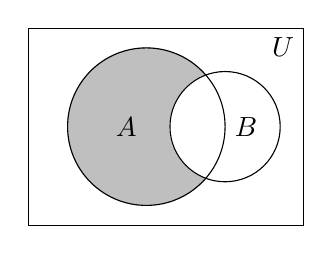
\begin{tikzpicture}
\draw (0,0) rectangle (3.5,2.5) node [below left] {$U$};
\filldraw [gray!50] (1.5,1.25) circle (1);
\filldraw [white] (2.5,1.25) circle (0.7);
\draw (1.5,1.25) circle (1) node [left] {$A$};
\draw (2.5,1.25) circle (0.7) node [right] {$B$};
\end{tikzpicture}\\
(2) 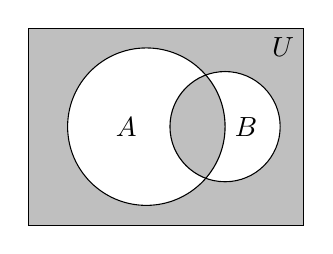
\begin{tikzpicture}
\filldraw [gray!50] (0,0) rectangle (3.5,2.5);
\draw (0,0) rectangle (3.5,2.5) node [below left] {$U$};
\filldraw [white] (1.5,1.25) circle (1);
\filldraw [white] (2.5,1.25) circle (0.7);
\begin{scope}
    \clip (1.5,1.25) circle (1);
    \clip (2.5,1.25) circle (0.7);
    \filldraw [gray!50] (0,0) rectangle (3.5,2.5);
\end{scope}
\draw (1.5,1.25) circle (1) node [left] {$A$};
\draw (2.5,1.25) circle (0.7) node [right] {$B$};
\end{tikzpicture}\\
(3) 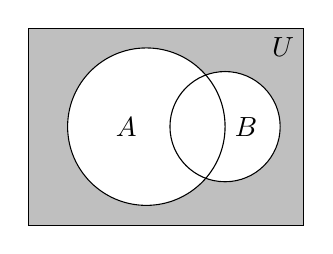
\begin{tikzpicture}
\filldraw [gray!50] (0,0) rectangle (3.5,2.5);
\draw (0,0) rectangle (3.5,2.5) node [below left] {$U$};
\filldraw [white] (1.5,1.25) circle (1);
\filldraw [white] (2.5,1.25) circle (0.7);
\draw (1.5,1.25) circle (1) node [left] {$A$};
\draw (2.5,1.25) circle (0.7) node [right] {$B$};
\end{tikzpicture}
\item 设全集为$U$, 且$M\subseteq N$, 则\blank{50}(填入所有正确选项的序号).\\
\textcircled{1} $M\cup N=N$; \textcircled{2} $M\cup N=M$; \textcircled{3} $\overline{N}\subseteq\overline{M}$ \textcircled{4} $\overline{M}\subseteq\overline{N}$; \textcircled{5} $\overline{M}\cup\overline{N}=U$; \textcircled{6} $M\cap\overline{N}=\varnothing$; \textcircled{7} $\overline{M}\cap N=\varnothing$.
\item 已知全集$U=A\cup B=\{x|0\le x\le 10, \ x\in \mathbf{N}\}$, $A\cap\overline B=\{1, 3, 5, 7\}$. 则集合$B=$\blank{50}.
\item 若全集$U=\{(x,y)|x\in\mathbf{R},\ y\in\mathbf{R}\}$, 集合$A=\{(x,y)|\dfrac yx=1\}$, 集合$B=\{(x,y)|y\neq x\}$, 则$\overline{A\cup B}= $\blank{50}.
\item 如图, 已知集合$U$为全集, 分别用集合$A$、$B$、$C$的运算式表示下列图中的阴影部分.
\begin{center}
    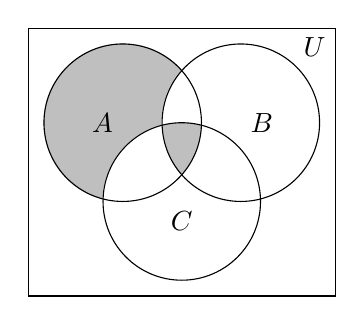
\begin{tikzpicture}
        \filldraw [gray!50] (0,0) circle (1);
        \filldraw [white] (1.5,0) circle (1);
        \filldraw [white] (0.75,-1) circle (1);
        \begin{scope}
            \clip (0,0) circle (1);
            \clip (1.5,0) circle (1);
            \clip (0.75,-1) circle (1);
            \filldraw [gray!50] (1.5,0) circle (1);
        \end{scope}
        \draw (0,0) circle (1) node [left] {$A$};
        \draw (1.5,0) circle (1) node [right] {$B$};
        \draw (0.75,-1) circle (1) node [below] {$C$};
        \draw (-1.2,-2.2) rectangle (2.7,1.2) node [below left] {$U$};
    \end{tikzpicture}
    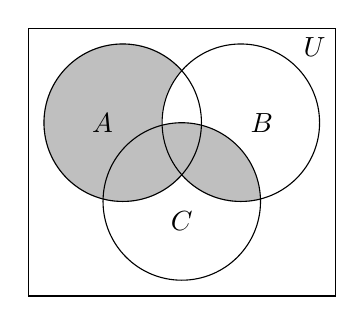
\begin{tikzpicture}
        \filldraw [gray!50] (0,0) circle (1);
        \filldraw [white] (1.5,0) circle (1);
        \begin{scope}
            \clip (0.75,-1) circle (1);
            \filldraw [gray!50] (1.5,0) circle (1);
        \end{scope}
        \draw (0,0) circle (1) node [left] {$A$};
        \draw (1.5,0) circle (1) node [right] {$B$};
        \draw (0.75,-1) circle (1) node [below] {$C$};
        \draw (-1.2,-2.2) rectangle (2.7,1.2) node [below left] {$U$};
    \end{tikzpicture}
\end{center}
\item 判断下列语句是否为命题, 并在相应的横线上填入``是''或``否''.\\
(1) 正方形和四边形;\blank{50};\\
(2) 正方形是四边形吗?\blank{50};\\
(3) $\pi>3$;\blank{50};\\
(4) 正方形好美!\blank{50};\\
(5) $2x>4$;\blank{50};\\
(6) $968$能被$11$整除;\blank{50}.
\item 判断下列命题的真假, 并在相应的括号内填入``真''或``假''.\\
(1) $2\sqrt 3>3\sqrt 2$或$1\le 1$;\blank{50};\\
(2) $2\sqrt 3>3\sqrt 2$且$1\le1$;\blank{50};\\
(3) 如果$a$、$b$都是奇数, 那么$ab$也是奇数;\blank{50};\\
(4) $\{1\}$是$\{0, 1, 2\}$的真子集;\blank{50};\\
(5) $1$是$\{0, 1, 2\}$的真子集;\blank{50};\\
(6) 若$x<-2$或$x>2$, 则$x^2>1$;\blank{50};\\
(7) 如果$|a|<2$, 那么$a<2$;\blank{50};\\
(8) 对任意实数$a,b$, 方程$(a+1)x+b=0$的解为$x=-\dfrac b{a+1}$;\blank{50};\\
(9) 若命题$\alpha$、$\beta$、$\gamma$满足$\alpha\Rightarrow \beta$, $\beta\Rightarrow \gamma$, $\gamma\Rightarrow \alpha$, 则$\alpha\Leftrightarrow \gamma$;\blank{50};\\
(10) 若关于$x$的方程$ax^2+bx+c=0$($a\ne 0$)的两实数根之积是正数, 则$ac>0$;\blank{50};\\
(11) 若某个整数不是偶数, 则这个数不能被$4$整除;\blank{50};\\
(12) 合数一定是偶数;\blank{50};\\
(13) 所有的偶数都是素数或合数;\blank{50};\\
(14) 所有的偶数都是素数或所有的偶数都是合数;\blank{50};\\
(15) 如果$A\subset B$, $B\supset C$, 那么$A=C$;\blank{50};\\
(16) 空集是任何集合的真子集;\blank{50};\\
(17) 若$x\in \mathbf{R}$, 则方程$x^2-x+1=0$不成立;\blank{50};\\
(18) 若$A\cap B\ne \varnothing$, $B\subset C$, 则$A\cap C\ne \varnothing$;\blank{50};\\
(19) 存在一个三角形, 它的任意两边的平方和小于第三边的平方;\blank{50};\\
(20) 对于任意一个三角形, 存在一组两边的平方和不等于第三边的平方;\blank{50}.
\item 在下列各题中, 用符号``$\Rightarrow$''``$\Leftarrow$''``$\Leftrightarrow$''把$\alpha$和$\beta$联系起来:\\
(1) $\alpha:a=0$, $\beta:ab=0$; $\alpha$\blank{20}$\beta$;\\
(2) $\alpha:x^2=4$, $\beta:x=2$; $\alpha$\blank{20}$\beta$;\\
(3) $\alpha:$实数$x$适合$x^2-5x+6=0$, $\beta:x=2$; $\alpha$\blank{20}$\beta$;\\
(4) $\alpha:\sqrt {x^2}=x$, $\beta:x>0$; $\alpha$\blank{20}$\beta$;\\
(5) $\alpha:$实数$x$适合$\dfrac{x-3}{x+1}=-1$, $\beta:x=1$; $\alpha$\blank{20}$\beta$;\\
(6) $\alpha:k$除以$4$余$1$, $\beta:k$除以$2$余$1$; $\alpha$\blank{20}$\beta$;\\
(7)$\alpha: \{2\}\subset B\subseteq \{2, 3, 5\}$, $\beta:B=\{2, 5\}$; $\alpha$\blank{20}$\beta$.
\item 已知命题``非空集合$M$的元素都是集合$P$的元素$''$是假命题, 给出下列命题: \textcircled{1} $M$中的元素都不是$P$的元素; \textcircled{2} $M$中有不属于$P$的元素; \textcircled{3} $M$中有$P$的元素; \textcircled{4} $M$中的元素不都是$P$的元素. 其中真命题有\blank{50}.
\item 已知$\alpha: 2\le x<4$, $\beta: 3m-1\le x\le-m$, 且$\alpha\Rightarrow\beta$, 求实数$m$的取值范围.
\item 已知$a$是常数, 命题$\alpha :-1<a<3$, $\beta$: 关于$x$的方程$x+a=0$($x\in \mathbf{R}$)没有正根, 若命题$\alpha$、$\beta$有且只有一个是真命题, 求实数$a$的取值范围.
\item 下列各题中$P$是$Q$的什么条件?(充分非必要、必要非充分、充要、既非充分又非必要)\\
(1) $P$: $x$是$2$的倍数, $Q$: $x$是$6$的倍数;\blank{50};\\
(2) $P$: $x$不是$2$的倍数, $Q$: $x$不是$6$的倍数;\blank{50};\\
(3) $P$: $x\in A$或$x\in B$, $Q$: $x\in A\cap B$;\blank{50};\\
(4) $P$: $f(x)=ax^2+bx+c$的图像过原点, $Q$: $c=0$;\blank{50}.
item 若$x,y,z$都是实数, 则:(填写``充分非必要、必要非充分、充要、既非充分又非必要''之一)\\
(1) ``$xy=0$''是``$x=0$''的\blank{50}条件;\\
(2) ``$x\cdot y=y\cdot z$''是``$x=z$''的\blank{50}条件;\\
(3) ``$\dfrac xy=\dfrac yz$''是``$xz=y^2$''的\blank{50}条件;\\
(4) ``$|x |>| y|$''是``$x>y>0$''的\blank{50}条件;\\
(5) ``$x^2>4$''是``$x>2$'' 的\blank{50}条件;\\
(6) ``$x=-3$''是``$x^2+x-6=0$'' 的\blank{50}条件;\\
(7) ``$|x+y|<2$''是``$|x|<1$且$|y|<1$'' 的\blank{50}条件;\\
(8) ``$|x|<3$''是``$x^2<9$'' 的\blank{50}条件;\\
(9) ``$x^2+y^2>0$''是``$x\ne 0$'' 的\blank{50}条件;\\
(10) ``$\dfrac{x^2+x+1}{3x+2}<0$''是``$3x+2<0$'' 的\blank{50}条件;\\
(11) ``$0<x<3$''是``$|x-1|<2$'' 的\blank{50}条件.
\item 如果$A$是$B$的必要条件, $C$是$B$的充分条件, $A$是$C$的充分条件, 那么$B$、$C$分别是$A$的\blank{50}和\blank{50}条件.
\item 写出使得``$x>3$''成立的一个充分条件: \blank{50}和一个必要条件: \blank{50}.
\item 一次函数$y=kx+b$的图像经过第二、三、四象限的一个充要条件是\blank{50}.
\item 关于$x$的方程$ax^2=0$至少有一个实数根的一个充要条件是\blank{50}.
\item 已知$x,y\in \mathbf{R}$, ``$x^2+y^2>0$''是``$x\ne 0$或$y\ne 0$''的\bracket{20}.
\twoch{充分而不必要条件}{必要而不充分条件}{充要条件}{既不充分又不必要条件}
\item 三个数$a$、$b$、$c$不全为零的充要条件是\bracket{20}.
\twoch{$a,b,c$都不是零}{$a,b,c$中最多一个零}{$a,b,c$中只有一个是零}{$a,b,c$中至少有一个不是零}
\item 证明: $x_1>2$且$x_2>2$是$x_1+x_2>4$且$x_1\cdot x_2>4$的充分非必要条件.
\item 有限集合$S$中元素的个数记作$\mathrm{card}(S)$, 设$A,B$都是有限集合, 给出下列命题:\\
\textcircled{1} $A\cap B=\varnothing$的一个充要条件是$\mathrm{card}(A\cup B)=\mathrm{card}(A)+\mathrm{card}(B)$;\\
\textcircled{2} $A\subseteq B$的一个必要不充分条件是$\mathrm{card}(A)\le \mathrm{card}(B)$; \\
\textcircled{3} $A$不是$B$的子集的一个充分不必要条件是$\mathrm{card}(A)>\mathrm{card}(B)$;\\ 
\textcircled{4} $A=B$的一个充要条件是$\mathrm{card}(A)=\mathrm{card}(B)$.\\ 
其中真命题的个数是\bracket{20}.
\fourch{$0$}{$1$}{$2$}{$3$}
\item 设$\alpha,\beta$是方程$x^2-ax+b=0$的两个实数根. 试分析$a>2$且$b>1$是``两个实数根$\alpha,\beta$均大于$1$''的什么条件? 并证明你的结论.
\item 设$x,y\in \mathbf{R}$, 求证: $|x+y|=|x|+|y|$成立的充要条件是$xy\ge 0$.
\item 已知下列字母均为常实数, 写出下列陈述句的否定形式;
(1) $x>0$; \blank{100};\\
(2) $1>x>0$; \blank{100};\\
(3) $x>0$且$y\le 1$; \blank{100};\\
(4) $x>0$或$x\le -2$; \blank{100};\\
(5) $x\ne y$或$y\ne z$; \blank{100};\\
(6) $a,b,c,d$中至多有$2$个$0$; \blank{100};\\
(7) $a,b,c,d$中至少有$2$个$1$; \blank{100};\\
(8) $a,b,c,d$都大于$1$; \blank{100};\\
(9) $a,b,c,d$不都大于$1$; \blank{100};\\
(10) $a,b,c,d$都不大于$1$; \blank{100}. 
\item 在横线上写出下列命题的否定形式, 并判断命题真假, 在相应的位置中填入``真''或``假''.\\
(1) $\pi$是无理数; \blank{20}; \blank{150}; \blank{20};\\
(2) $2+1=4$;  \blank{20}; \blank{150}; \blank{20};\\
(3) 任何实数是正数或负数;  \blank{20}; \blank{150}; \blank{20};\\
(4) 任何实数是正数或任何实数是负数;  \blank{20}; \blank{150}; \blank{20};\\
(5) 对一切实数$x, x^3+1=0$;  \blank{20}; \blank{150}; \blank{20};\\
(6) 存在实数$x, x^3+1=0$;  \blank{20}; \blank{150}; \blank{20};\\
(7) 对于任意实数$k$, 关于$x$的方程$x^2+x+k=0$都有实数根;  \blank{20}; \blank{250}; \blank{20};\\
(8) 任何三角形中至多有一个钝角;  \blank{20}; \blank{150}; \blank{20};\\
(9) 若$a>1$, $b>1$, 则$ab>1$;  \blank{20}; \blank{150}; \blank{20};\\
(10) 能被$2$整除的整数是质数;  \blank{20}; \blank{150}; \blank{20}.\\
\item 写出下列命题的否定形式.\\
(1) 在平面上, 过定点$P$有且只有一条直线垂直于给定直线$l$;\\
(2) 任意两个有理数之间存在一个无理数;\\
(3) 存在实数$a$, 使得关于$x$的不等式$x^2+(a-2)x+a-1\ge 0$至少有一个正数解;\\
(4) 存在实数$a$, 使得关于$x$的不等式$x^2+(a-2)x+a-1\ge 0$恒成立;\\
(5) 存在实数$a$, 使得关于$x$的不等式$x^2+(a-2)x+a-1\ge 0$有解.
\item 已知甲$\Rightarrow$乙, 下列说法一定正确的是\bracket{20}.
\twoch{甲不成立, 可推出乙成立}{甲不成立, 可推出乙不成立}{乙不成立, 可推出甲成立}{乙不成立, 可推出甲不成立}
\item ``$a\ne 1$且$b\ne 2$''是``$a+b\ne 3$''的\bracket{20}.
\twoch{充分非必要条件}{必要非充分条件}{充要条件}{既非充分又非必要条件}
\item 证明: 若$x+2y+z>0$, 则$x,y,z$中至少有一个大于$0$.
\item 证明:对于三个实数$a,b,c$, 若$a\ne c$, 则$a\ne b$或$b\ne c$.
\item ``$x\ne 3$或$x\ne 4$'' 是``$x^2-7x+12\ne 0$''的\bracket{20}.
\twoch{充分非必要条件}{必要非充分条件}{充要条件}{既非充分又非必要条件}
\item 证明: 若$x^2\ne y^2$, 则$x\ne y$或$x\ne -y$.
\item 若$a^3+b^3=2$, 证明: $a+b\le 2$.


\end{enumerate}

\end{document}